\chapter{Genome assembly of Candida nivariensis}
\label{chap:rnw}





This document was generated on Mon May  2 16:13:51 2022.

As shown in Figure \ref{fig:mummer} and in Table \ref{tab:rtab1} we can see that bla bla \citep{B}.


\begin{figure}[!ht]
\centering
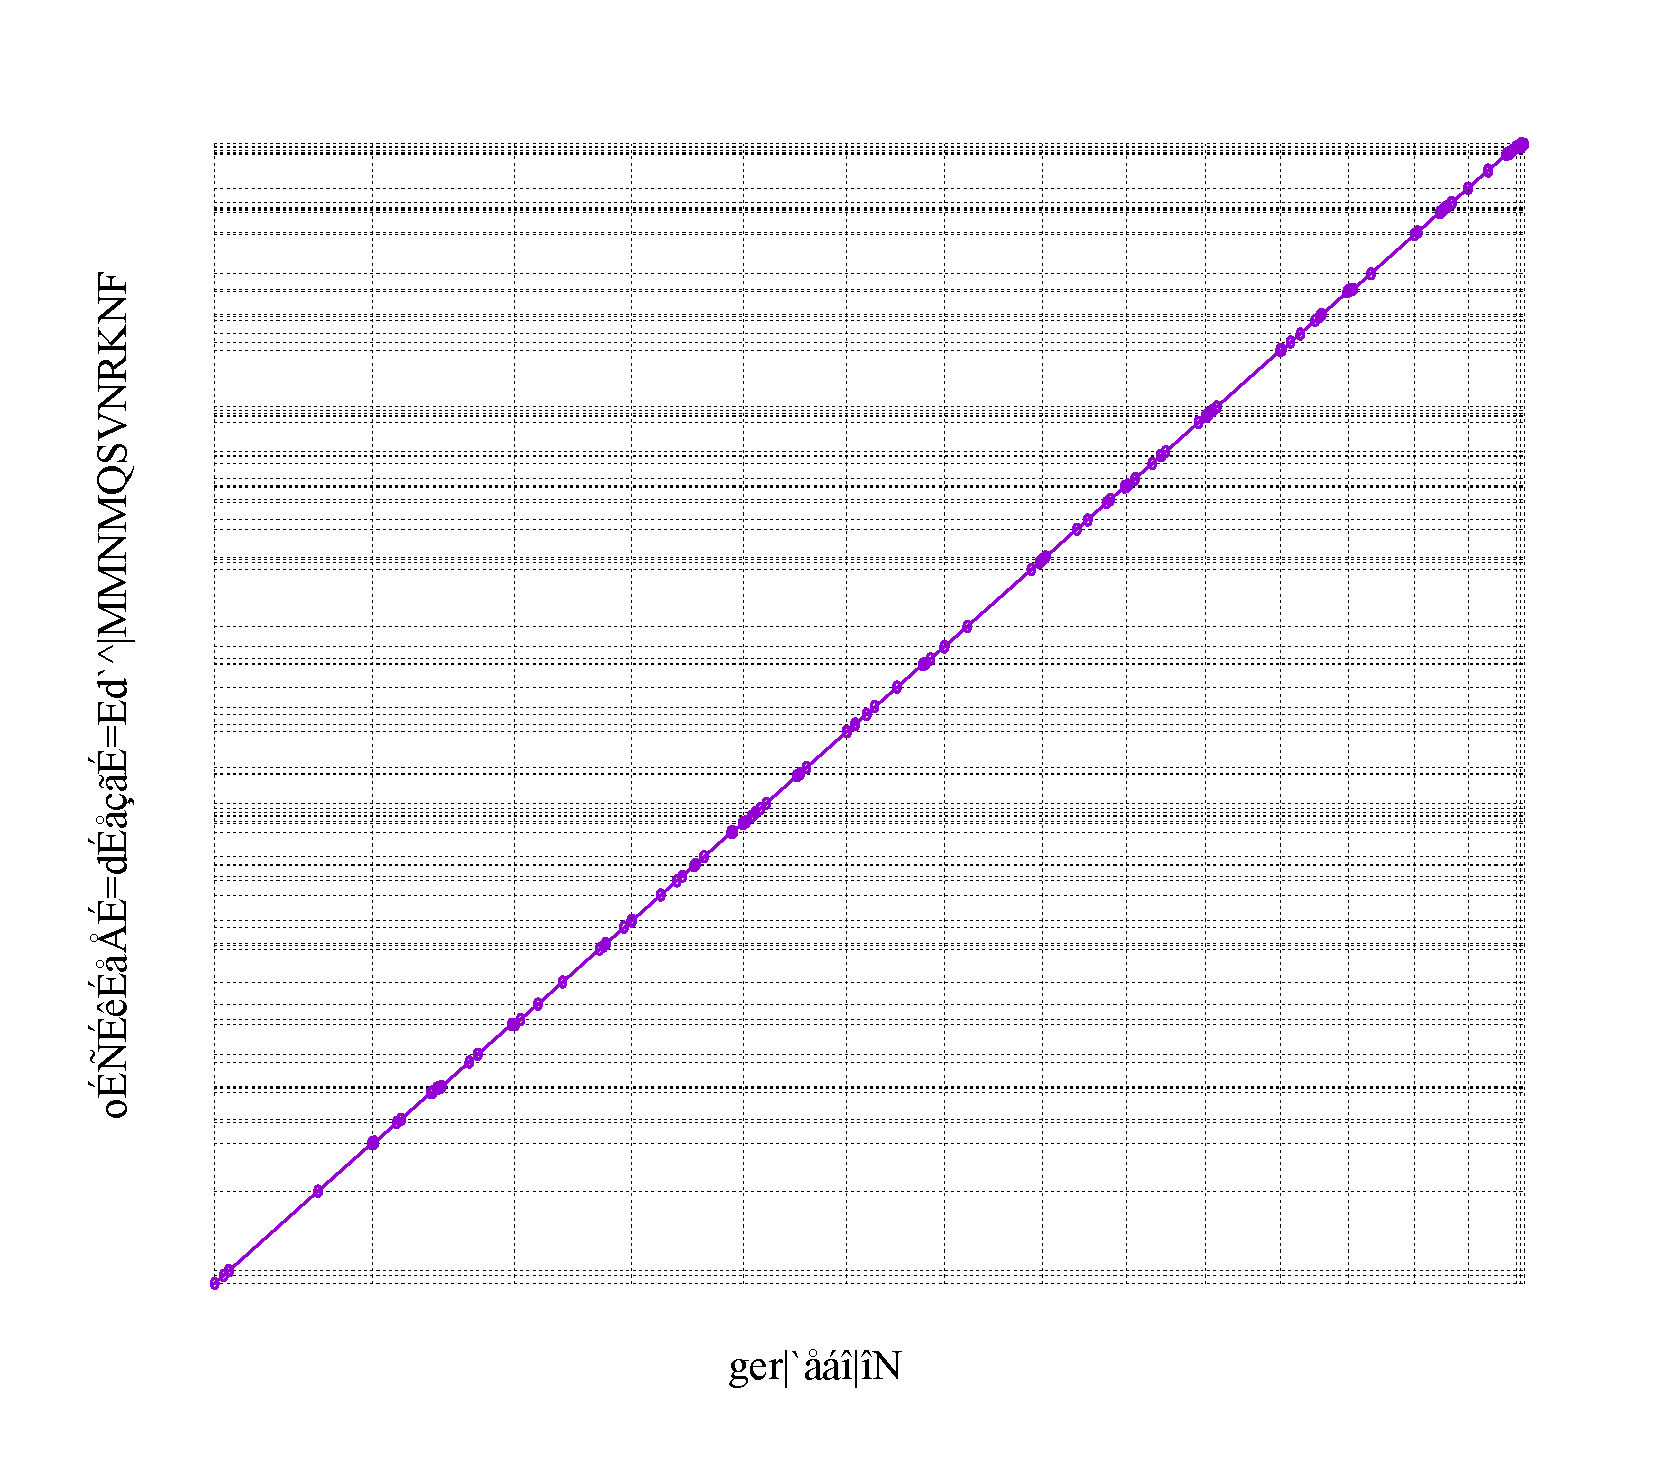
\includegraphics[width = 1\linewidth,keepaspectratio]{figure/mummer.pdf}
\caption[Mummer between stuff]{{\bf Mummer between stuff.} {\bf (a)} blah first point {\bf (b)} blah second point {\bf (c)} blaih thrid panel  }
\label{fig:mummer}
\end{figure}




% latex table generated in R 3.6.3 by xtable 1.8-4 package
% Mon May  2 16:13:51 2022
\begin{table}[ht]
\centering
\begin{tabular}{rr}
  \hline
A & B \\ 
  \hline
  1 & 0.00 \\ 
    2 & 0.16 \\ 
    3 & -0.56 \\ 
    4 & -1.40 \\ 
    5 & 0.05 \\ 
    6 & 0.06 \\ 
    7 & 1.08 \\ 
    8 & 0.14 \\ 
    9 & -2.29 \\ 
   10 & 0.02 \\ 
   \hline
\end{tabular}
\caption{\bf{ Table title } Table description} 
\label{tab:rtab1}
\end{table}

